\begin{name}
	{ÔN TẬP KIỂM TRA GIỮA HỌC KÌ 1}
	{TOÁN 10}
	{LỚP TOÁN THẦY PHÁT}
	{\thoigian}
\end{name}

\caulc

\Opensolutionfile{ans}[ans-ABCD]
\begin{ex}%[0D1N1-1]%[KNTT - Lớp 10 - Ôn tập giữa học kì 1 - Đề 2]%[Phamhaiduong]
	Trong các câu sau, câu nào là mệnh đề Toán học?
	\def\dotEX{}
	\choice
	{Hoa Bỉ Ngạn xanh nở vào buổi sáng.}
	{\True Số $6$ là số chẵn.}
	{Mèo Orgy có màu xanh.}
	{Các bạn có làm được bài kiểm tra này không?}
	\loigiai{
		Số 6 là số chẵn là câu khẳng định đúng nên là mệnh đề.
	}
\end{ex}

\begin{ex}%[0D1H1-5]%[KNTT - Lớp 10 - Ôn tập giữa học kì 1 - Đề 2]%[Phamhaiduong]
	Tìm mệnh đề đúng.
	\choice
	{\True $\forall n \in \mathbb{N}\colon n(n+1)(n+2)$ chia hết cho $6$}
	{$\forall n \in \mathbb{N}\colon n^2 + 1$ là số lẻ}
	{$\exists x \in \mathbb{R}\colon x^2 < 0$}
	{$\forall x \in \mathbb{R}\colon x^2 = x$}
	\loigiai
	{\begin{itemize}
			\item  $\forall n \in \mathbb{N}\colon n(n+1)(n+2)$ chia hết cho $6$ đúng vì $n(n+1)(n+2)$ là tích 3 số tự nhiên liên tiếp nên chia hết cho 6.
			\item  $\forall n \in \mathbb{N}\colon n^2 + 1$ là số lẻ sai vì với $n=3$ thì $n^2 + 1 = 3^2 + 1 = 10$ là số chẵn.
			\item  $\exists x \in \mathbb{R}\colon x^2 < 0$ sai vì $x^2 \geq 0$, $\forall x \in \mathbb{R}$.
			\item  $\forall x \in \mathbb{R}\colon x^2 = x$ sai vì với $x=2$ thì $x^2 \neq x$.
		\end{itemize}
	}
\end{ex}

\begin{ex}%[0D1N1-4]%[KNTT - Lớp 10 - Ôn tập giữa học kì 1 - Đề 2]%[Phamhaiduong]
	Cho mệnh đề \lq\lq$A \Rightarrow B$\rq\rq. Phát biểu nào sau đây \textbf{không }thay thế cho phát biểu trên?
	\choice
	{Nếu $A$ thì $B$}
	{\True Nếu $B$ thì $A$}
	{$A$ suy ra $B$}
	{$A$ là điều kiện đủ để có $B$}
	\loigiai{
		Theo lí thuyết thì Nếu $B$ thì $A$ là phát biểu không thay thế cho mệnh đề đã cho.
	}
\end{ex}

\begin{ex}%[0D1N2-3]%[KNTT - Lớp 10 - Ôn tập giữa học kì 1 - Đề 2]%[Phamhaiduong]
	\immini{Hình vẽ bên biểu diễn cho tập hợp nào trên trục số?}{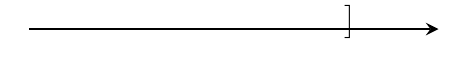
\begin{tikzpicture}[>=stealth,line width=1pt]
			\draw[->](-4,0)->(1.2,0);		%Vẽ trục số
			\def\skipInterval{0.5cm}		%Khoảng cách đặt nhãn
			% \def\colorInterval{blue} 	%Màu tick, màu fill miền
			\Interval{\big]}{-2}{}{ }

		\end{tikzpicture}
	}
	\choice
	{$(-\infty;-2)$}
	{\True $(-\infty;-2]$}
	{$[-2;+\infty)$}
	{$(-2;+\infty)$}
	\loigiai
	{Theo định nghĩa ta có $(-\infty;-2]$.
	}
\end{ex}

\begin{ex}%[0D1H3-1]%[KNTT - Lớp 10 - Ôn tập giữa học kì 1 - Đề 2]%[Phamhaiduong]
	Cho hai tập hợp $A = \{x \in \mathbb{Z} | (x^2 - 10x + 21)(x^3 - x) = 0\}$, $B = \{x \in \mathbb{Z} | -3 < 2x - 1 < 5\}$. Khẳng định nào sau đây là đúng?
	\choice{$A \cap B = \varnothing$}
	{$A \cap B = \{-1; 3; 7\}$}
	{$A \cup B = \{0; 1\}$}
	{\True $A \cup B = \{-1; 0; 1; 2; 3; 7\}$}
	\loigiai{Ta có
		$(x^2 - 10x + 21)(x^3 - x) = 0 \Leftrightarrow\hoac{&(x - 3)(x - 7) = 0 \\& x(x^2 - 1) = 0} \Leftrightarrow x \in \{-1; 0; 1; 3; 7\}$.\\
		Giải bất phương trình $-3 < 2x - 1 < 5 \Leftrightarrow -1 < x < 3$, mà $x \in \mathbb{Z}$ nên $B = \{0; 1; 2\}$.\\
		Khi đó $A \cap B=\{0;1\}$, $A \cup B = \{-1; 0; 1; 2; 3; 7\}$.
	}
\end{ex}

\begin{ex}%[De-chuan-hoa-so-6]%[Đình Nguyên]%[0H4N1-1]
	Cho góc $\alpha\left(0^\circ<\alpha<180^\circ\right)$. Khẳng định nào sau đây là đúng?
	\choice
	{\True $-1<\cos \alpha<1$}
	{$-1<\cot \alpha<1$}
	{$-1<\tan \alpha<1$}
	{$0<\sin \alpha<1$}
	\loigiai{
		Vì $0^\circ<\alpha<180^\circ$ nên $-1<\cos \alpha<1$ và $0< \sin \alpha \le 1$.
	}
\end{ex}

\begin{ex}%[Dự án EX-10-11-Chuẩn hóa]%[Hoàng Thanh Phương]%[0H4N1-2]
	Trong các đẳng thức sau đây, đẳng thức nào đúng?
	\choice
	{\True $\tan 150^\circ=-\dfrac{\sqrt{3}}{3}$}
	{$\cos 150^\circ=\dfrac{\sqrt{3}}{2}$}
	{$\sin 150^\circ=-\dfrac{\sqrt{3}}{2}$}
	{$\cot 150^\circ=\sqrt{3}$}
	\loigiai{
		Ta có 	$\tan 150^\circ=-\dfrac{\sqrt{3}}{3}$.
	}
\end{ex}

\begin{ex}%[HKI, Phan Bội Châu- Bình Thuận, 2023]%[Hiếu Phan]%[0H4N2-1]
	Cho tam giác $ABC$ với $BC=a,\,CA=b,\,AB=c.$ Mệnh đề nào sau đây là \textbf{sai}?
	\choice
	{$c=\dfrac{a\sin C}{\sin A}$}
	{\True $a=\dfrac{c\sin A}{\sin B}$}
	{$b=\dfrac{a\sin B}{\sin A}$}
	{$a=\dfrac{b\sin A}{\sin B}$}
	\loigiai{
		Theo định lý sin ta có  $\dfrac{a}{\sin A}=\dfrac{c}{\sin C}\Rightarrow a=\dfrac{c\sin A}{\sin C}$ nên $a=\dfrac{c\sin A}{\sin B}$ sai.
	}
\end{ex}

\begin{ex}%[0H4N2-2]%[KNTT - Lớp 10 - Ôn tập giữa học kì 1 - Đề 2]%[Phamhaiduong]
	Cho tam giác ABC có $AB = AC = b$, $CB = a$, $p = \dfrac{a+b+c}{2}$. Diện tích $S$ của tam giác $ABC$ được tính theo công thức nào sau đây?
	\choice{$S = p\sqrt{p(p+a)(p+b)(p+c)}$}
	{$S = \dfrac{1}{2}ac \cos A$}
	{$S = bc \cos A$}
	{\True $S = \sqrt{p(p-a)(p-b)(p-c)}$}
	\loigiai{
		Ta có $S = \sqrt{p(p-a)(p-b)(p-c)}$.
	}
\end{ex}

\begin{ex}%[0D2N1-2]%[KNTT - Lớp 10 - Ôn tập giữa học kì 1 - Đề 2]%[Phamhaiduong]
	Cho bất phương trình $2x + y \leq 3$. Miền nghiệm của bất phương trình trong mặt phẳng tọa độ $Oxy$ là
	\choice
	{Nửa mặt phẳng chứa điểm $O$ có bờ là đường thẳng $2x + y = -3$}
	{Nửa mặt phẳng không chứa điểm $O$ có bờ là đường thẳng $2x + y = -3$}
	{\True Nửa mặt phẳng chứa điểm $O$ có bờ là đường thẳng $2x + y = 3$}
	{Nửa mặt phẳng không chứa điểm $O$ có bờ là đường thẳng $2x + y = 3$}
	\loigiai{
		Vì bất phương trình có dấu $\leq$ nên kể cả bờ.
		Thay $x = 0$, $y = 0$ vào bất phương trình ta thấy miền nghiệm chứa $O$.
	}
\end{ex}
\begin{ex}%[0D2N2-1]%[KNTT - Lớp 10 - Ôn tập giữa học kì 1 - Đề 2]%[Phamhaiduong]
	Cặp số $(x; y)$ nào sau đây là nghiệm của hệ bất phương trình $\heva{&2x+y>0\\ &x-y-2\le0}$?
	\choice{$(0;0)$}
	{$(-2;4)$}
	{\True $(3;4)$}
	{$(0;-3)$}
	\loigiai{
		Thay lần lượt $(x; y)$ bởi các cặp số trong đáp án ta thấy $(3;4)$ là nghiệm của hệ bất phương trình.
	}
\end{ex}
\begin{ex}%[0D2H1-2]%[KNTT - Lớp 10 - Ôn tập cuối học kì 1 - Đề 03]%[Nguyễn Hữu Chung Kiên]
	\immini[thm]{Đường thẳng $d\colon 2x-y-2=0$ chia mặt phẳng tọa độ thành hai miền $I$, $II$ là hai nửa mặt phẳng có bờ là đường thẳng $d$ (tham khảo hình vẽ bên). Xác định miền nghiệm của bất phương trình $2x-y-2\ge 0$.
		\choice
		{Nửa mặt phẳng $I$ bỏ đi đường thẳng $d$}
		{\True Nửa mặt phẳng $I$ kể cả bờ $d$}
		{Nửa mặt phẳng $II$ kể cả bờ $d$}
		{Nửa mặt phẳng $II$ bỏ đi đường thẳng $d$}}
	{\begin{tikzpicture}[line join=round, line cap=round,>=stealth,thick,scale=0.7]
			\tikzset{every node/.style={scale=0.9}}
			\draw[->] (-3.1,0)--(5.1,0) node[below left] {$x$};
			\draw[->] (0,-3.1)--(0,4.1) node[below left] {$y$};
			\draw (0,0) node [below left] {$O$};
			\draw (3,2) node [below left] {$I$};
			\draw (1.6,3) node [below left] {$II$};
			\draw (2.5,3.8) node [below left] {$d$};
			\foreach \x/\nx in {1/1}
			\draw[thin] (\x,1pt)--(\x,-1pt) node [below] {$\nx$};
			\foreach \y/\ny in {-2/-2}
			\draw[thin] (1pt,\y)--(-1pt,\y) node [left] {$\ny$};
			\begin{scope}
				\clip (-3,-3) rectangle (5,4);
				\draw[samples=200,domain=-2:4,smooth,variable=\x] plot (\x,{2*(\x)+-2});
			\end{scope}
		\end{tikzpicture}}
	\loigiai{Ta thấy $O(0; 0) \notin d$ và $2\cdot0 - 0 - 2 = -2 < 0$ nên $(0; 0)$ \textbf{không} là nghiệm của bất phương trình $2x - y - 2 \ge 0$. \\
		Do đó miền nghiệm của bất phương trình $2x - y - 2 \ge 0$ là miền không chứa điểm $O$ kể cả đường thẳng $d$. \\
		Vậy miền nghiệm của bất phương trình $2x - y - 2 \ge 0$ là nửa mặt phẳng $I$ kể cả bờ $d$.}
\end{ex}
\Closesolutionfile{ans}
% % \indapan{6}{ans-ABCD}
\cauds
\Opensolutionfile{ans}[ans-DS]

\begin{ex}%[0D1V1-2]%[KNTT - Lớp 10 - Ôn tập giữa học kì 1 - Đề 2]%[phamhaiduong]
	Cho biểu thức $P(n)=-3 n^2+2n+5$. Tập hợp $A=\{x \in \mathbb{R} \mid -2 \le x \le 4\}$, $B=\{n \in \mathbb{N} \mid P(n) =0\}$.
	\choiceTF
	{\True $A=[-2;4]$}
	{Tập hợp $B$ có tất cả $4$ tập con}
	{\True $A \cap B = \varnothing$}
	{\True Tồn tại số tự nhiên $n$ để biểu thức $\dfrac{P(n)+n+1}{n-1}$ có giá trị nguyên}
	\loigiai{
		\begin{itemchoice}
			\itemch $A=\{x \in \mathbb{R} \mid -2 \le x \le 4\} = [-2;4]$.
			\itemch $P(n)=-3 n^2+2n+5=0 \Leftrightarrow n = -1 \text{ hoặc } n = \dfrac{5}{3}$.\\
			Vì $n\in \mathbb{N}$ nên $B=\varnothing$.\\
			Tập hợp $B$ chỉ có $1$ tập con là $\varnothing$.
			\itemch Vì $B = \varnothing$ nên $A \cap B=\varnothing$.
			\itemch Ta có $\dfrac{P(n)+n+1}{n-1}=\dfrac{-3 n^2+3 n+6}{n-1}=-3 n + \dfrac{6}{n-1}$.\\
			$\dfrac{P(n)+n+1}{n-1}$ có giá trị nguyên khi $n-1$ là ước của $6$.\\
			Suy ra $n-1 \in \{-6;-3;-2;-1;1;2;3;6\} \Rightarrow n \in \{0;2;3;4;7\} \subset \mathbb{N}$.\\
			Vậy có tồn tại số tự nhiên $n$ để biểu thức $\dfrac{P(n)+n+1}{n-1}$ có giá trị nguyên.
		\end{itemchoice}
	}
\end{ex}
\begin{ex}%[Mức 3]%[Dự án Giảng 10, 11, Huỳnh Quy]%[0D2V2-3]
	Người trưởng thành trung bình cần tối thiểu $ 0{,}8 $ g protein cho mỗi kg trọng lượng cơ thể mỗi ngày (lời khuyên từ WHO). Trong $ 100 $ g cá ngừ có $ 26 $ g protein, $ 100 $ g tôm có $ 18 $ g protein.\\
	\textit{(Nguồn: https://ifitness.vn)}\\
	Gọi $ x $, $ y $ lần lượt là số lạng cá ngừ và số lạng tôm mà một người trưởng thành nặng $ 75 $ kg ăn trong một ngày. Biết rằng người này chỉ mua nhiều nhất $ 1{,}5 $ kg cá ngừ và $ 4{,}5 $ kg tôm. Giá tiền một kg cá ngừ là $ 250 $ nghìn đồng, một kg tôm là $ 180 $ nghìn đồng. Các khẳng định sau đây đúng hay sai?
	\choiceTF[t]
	{Điều kiện của $x$ là $0\leq x\leq 1{,}5$}
	{Số tiền cần phải trả là $18x+25y$ (nghìn đồng)}
	{\True Bất phương trình bậc nhất hai ẩn $ x $, $ y $ biểu diễn lượng protein cần thiết trong một ngày của người đó là $13x+9y\geq 30$}
	{\True Để đảm bảo lượng protein cần thiết mà phải trả tiền ít nhất thì người đó cần mua $ 1{,}5$ lạng cá ngừ và $\dfrac{7}{6}$ lạng tôm}
	\loigiai{
		\begin{itemchoice}
			\itemch Do người này chỉ mua nhiều nhất là $1{,}5$ kg $=15$ lạng cá ngừ nên ta có $0\leq x\leq 15$.
			\itemch Số tiền phải trả là $T=25x+18y$ (nghìn đồng).
			\itemch Điều kiện $0\leq x\leq 15$, $0\leq y\leq 45$.\\
			Người trưởng thành nặng $ 75 $ kg cần tối thiểu $ 0{,}8\cdot 75= 60$ g protein.
			Theo giả thiết ta có $26x+18y\geq 60 \Leftrightarrow 13x+9y\geq 30$.
			\itemch 
			\immini{
			Xét hệ phương trình \[\heva{&13x+9y\geq 30&\quad(1)&\\&0\leq x\leq 15 &\quad(2)&\\&0\leq y\leq 45&\quad(3)&.}\]
			Miền nghiệm của hệ bất phương trình là miền đa giác $ABCDE$ như hình vẽ (tức là miền không gạch sọc (kể cả bờ)) với $A\left(0;\dfrac{10}{3} \right)$, $B\left(\dfrac{30}{13};0 \right)$, $C\left(15;0 \right)$ và $D\left(15;45 \right)$, $E(0;45)$.\\
			Ta có $T\left(0;\dfrac{10}{3} \right)=60$, $T\left(\dfrac{30}{13};0 \right)\approx 57{,}7$, \ldots\\
			Suy ra $\min T=57{,}7$ khi $x=\dfrac{10}{3}\approx 3,3$ và $y=0$.\\
			Vậy người đó mua $ 3,3$ lạng cá ngừ và $ 0$ lạng tôm để số tiền phải trả ít nhất mà vẫn đảm bảo lượng protein cần thiết.}{\begin{tikzpicture}[>=stealth,line join=round,line cap=round,font=\footnotesize,scale=.6,x=1cm,y=1cm]
				\def\xmin{-.5} \def\xmax{6}
				\def\ymin{-.5} \def\ymax{11}
				\path
				(0,3.3333) coordinate (A)
				(2.3077,0) coordinate (B)
				(5,0) coordinate (C)
				(5,10) coordinate (D)
				(0,10) coordinate (E)
				;
				\clip (\xmin,\ymin) rectangle (\xmax,\ymax);
				\fill[pattern = north west lines,pattern color = blue!50, smooth,opacity=0.5]
				(\xmin,\ymin)--plot[domain=\xmin:\xmax](\x,{3.3333-1.4444*\x})-- cycle;
				\fill[pattern = north west lines,pattern color = green!50, smooth,opacity=0.5]
				(\xmin,\ymin)rectangle(\xmax,0);
				\fill[pattern = north west lines,pattern color = red!50, smooth,opacity=0.5]
				(\xmin,\ymin)rectangle(0,\ymax);
				\fill[pattern = north west lines,pattern color = orange!50, smooth,opacity=0.5]
				(\xmin,\ymax)--plot[domain=\xmin:\xmax](\x,10)--(\xmax,\ymax)-- cycle;
				\fill[pattern = north west lines,pattern color = violet!50, smooth,opacity=0.5]
				(5,\ymin)rectangle(\xmax,\ymax);
				\foreach \x/\g in
					{A/45,B/45,C/-120,D/-135,E/-45}\fill[black]
				(\x) circle (1pt)
				($(\x)+(\g:3mm)$)node{$\x$};
				\draw (5,\ymin)--(5,\ymax) (\xmin,10)--(\xmax,10);
				\draw[->] (\xmin,0)--(\xmax,0) node [above left]{$x$};
				\draw[->] (0,\ymin)--(0,\ymax) node [below right]{$y$};
				\node at (0,0) [above right]{$O$};
				\node at (5,5) [below right]{$d_1$};
				\node at (3,10) [above left]{$d_2$};
				\node at (1,2.4) [above left]{$d$};
				\draw[color=blue,line width=0.5, smooth, samples=100, domain= -1:9] plot(\x,{3.3333-1.4444*\x});
			\end{tikzpicture}}
		\end{itemchoice}}
\end{ex}
\begin{ex}%[Mức độ 3]%[Nguyễn Trung Kiên, dự án giảng 10-11, CTGDPT2018]%[0H4V1-2]
	Cho góc $\alpha$ có $\sin\alpha=\dfrac{3}{5}$, $\tan\alpha=\dfrac{3}{4}$ và điểm $M$ nằm trên nửa đường tròn đơn vị sao cho $\widehat{xOM}=\alpha$.
	\choiceTF
	{$\cos\alpha=\dfrac{9}{20}$}
	{Điểm $M$ có tọa độ là $\left(\dfrac{3}{5};-\dfrac{4}{5}\right)$}
	{\True $\dfrac{\sin\alpha-\cos\alpha}{\sin\alpha+\cos\alpha}=-\dfrac{1}{7}$}
	{\True $2\sin\left(180^\circ-\alpha\right)-3\cos\left(90^\circ-\alpha\right) = -\dfrac{3}{5}$}
	\loigiai
	{\begin{itemchoice}
			\itemch Ta có $\tan\alpha=\dfrac{\sin\alpha}{\cos\alpha} \Leftrightarrow \cos\alpha=\dfrac{\sin\alpha}{\tan\alpha}=\dfrac{4}{5}$.
			\itemch Tọa độ điểm $M$ là $\left(\dfrac{4}{5};\dfrac{3}{5}\right)$.
			\itemch
			Ta có $\dfrac{\sin\alpha-\cos\alpha}{\sin\alpha+\cos\alpha} =\dfrac{\dfrac{3}{5}-\dfrac{4}{5}}{\dfrac{3}{5}+\dfrac{4}{5}} =\dfrac{-\dfrac{1}{5}}{\dfrac{7}{5}}=-\dfrac{1}{7}$.
			\itemch
			Ta có $2\sin\left(180^\circ-\alpha\right)-3\cos\left(90^\circ-\alpha\right) =2\sin\alpha -3\sin\alpha =-\sin\alpha =-\dfrac{3}{5}$.
		\end{itemchoice}}
\end{ex}
\Closesolutionfile{ans}
% % \indapan{3}{ans-DS}

\caukq
\Opensolutionfile{ans}[ans-KQ]

\begin{ex}%[0D1V3-3]%[KNTT - Lớp 10 - Ôn tập giữa học kì 1 - Đề 2]%[Phamhaiduong]
	Cho hai tập hợp khác rỗng $A=(m-1 ; 8]$ và $B=(-10 ; 2 m+2)$, $m \in \mathbb{R}$. Có bao nhiêu giá trị nguyên dương của tham số $m$ để $A \cap B \neq \varnothing$?
	\shortans{$8$}
	\loigiai{Điều kiện để hai tập $A=(m-1 ; 8]$ và $B=(-10 ; 2 m+2)$ khác tập rỗng là
		$$
			\heva{
				& m - 1 < 8  \\
				&2 m + 2 > - 1 0 } \Leftrightarrow \heva{
				&m<9 \\
				&m>-6
			} \Leftrightarrow-6<m<9\quad (*).
		$$
		Ta có $A \cap B \neq \varnothing \Leftrightarrow m-1<2 m+2 \Leftrightarrow m>-3$.\\
		Khi đó kết hợp điều kiện được có $8$ giá trị nguyên dương thoả mãn.
	}
\end{ex}

\begin{ex}%[0H4V3-2]%[KNTT - Lớp 10 - Ôn tập giữa học kì 1 - Đề 2]%[Phamhaiduong]
	\immini{
	Giả sử $CD=h$ là chiều cao của tháp trong đó $C$ là chân tháp. Chọn hai điểm $A, B$ trên mặt đất sao cho ba điểm $A$, $B$, $C$ thẳng hàng. Ta đo được $A B=24$ m, $\widehat{CAD}=63^{\circ}$, $\widehat{CBD}=48^{\circ}$. Tính chiều cao $h$ của tháp (làm tròn đến hàng phần chục).
	\shortans{$61{,}4$}
	}{
	\begin{tikzpicture}[>=stealth,line join=round,line cap=round,font=\footnotesize,scale=.6]
		\coordinate (C) at (0,0);

		\coordinate (A) at (5.5,0);

		\coordinate (B) at (7.5,0);

		\coordinate (D) at (0,7);

		\coordinate (v) at (1,0);
		\coordinate (M) at ($(D)-(2,0)$);

		\coordinate (N) at ($(C)-(2,0)$);

		\coordinate (P) at ($(B)+(1,0)$);

		\draw[<->, dashed] ($(C)-(1.5,0)$)--($(D)-(1.5,0)$) node[midway, left] {$h$};

		\draw[<->, dashed] ($(A)-(0,0.7)$)--($(B)-(0,0.7)$) node[midway, above] {$24$ m};

		\draw (N)--(v) (A)--(P) (A)--(D) (B)--(D);

		\draw[dashed] (M)--(D);

		\draw[pattern=north east lines] (1.5,-0.5) .. controls (1.5,-1.5) and (1.5,-2) .. (2.5,-2)

		.. controls (4,-2) and (4,-1) .. (4.5,-0.5)--cycle;

		\fill plot  coordinates{(0,0)(-1,0) (-0.63,0.77) (-0.4,0.77) (-0.4,5.05)(-0.63,5.05) (-0.63,5.53) (-0.45,5.53)(-0.22,6.24)(0,7)};

		\draw plot  coordinates{(1,0)(1,0) (0.63,0.77) (0.4,0.77) (0.4,5.05)(0.63,5.05) (0.63,5.53) (0.45,5.53)(0.22,6.24)(0,7)};

		\draw (1,0) .. controls (1.5,0) and (1.5,-0.5) .. (1.5,-0.5);

		\draw (4.5,-0.5) .. controls (4.5,-0.5) and (4.5,0) .. (5,0)--(A);

		\draw pic [draw,"$63^\circ$ ", angle eccentricity=1.5,angle radius =6 mm] {angle = D--A--C};

		\draw pic [draw,"$48^\circ$ ", angle eccentricity=1.5,angle radius =6 mm,double] {angle = D--B--C};
		\foreach \x/\g in {A/-90,B/-90,C/-90,D/90}\fill[black](\x)circle(1pt)+(\g:.3)node{$\x$};
	\end{tikzpicture}
	}
	\loigiai{\immini{Ta có $\widehat{C A D}=\widehat{C B D}+\widehat{A D B}$\\
	$\Rightarrow \widehat{A D B}=63^{\circ}-48^{\circ}=15^{\circ}$.\\
	Áp dụng định lí sin trong tam giác $A B D$ có $$\dfrac{A B}{\sin \widehat{A D B}}=\dfrac{A D}{\sin \widehat{A B D}}
		\Rightarrow A D=\dfrac{24 \cdot \sin 48^{\circ}}{\sin 15^{\circ}}=68{,}9.$$
	Trong tam giác vuông $A C D$ có $C D=A D \cdot \sin \widehat{A C D}=68{,}9 \cdot \sin 63^{\circ}=61{,}4(\mathrm{~m})$.\\
	Vậy $h=61{,}4$ m.}{	\begin{tikzpicture}[>=stealth,line join=round,line cap=round,font=\footnotesize,scale=.6]
		\coordinate (C) at (0,0);

		\coordinate (A) at (5.5,0);

		\coordinate (B) at (7.5,0);

		\coordinate (D) at (0,7);

		\coordinate (v) at (1,0);
		\coordinate (M) at ($(D)-(2,0)$);

		\coordinate (N) at ($(C)-(2,0)$);

		\coordinate (P) at ($(B)+(1,0)$);

		\draw[<->, dashed] ($(C)-(1.5,0)$)--($(D)-(1.5,0)$) node[midway, left] {$h$};

		\draw[<->, dashed] ($(A)-(0,0.7)$)--($(B)-(0,0.7)$) node[midway, above] {$24$ m};

		\draw (N)--(v) (A)--(P) (A)--(D) (B)--(D);

		\draw[dashed] (M)--(D);

		\draw[pattern=north east lines] (1.5,-0.5) .. controls (1.5,-1.5) and (1.5,-2) .. (2.5,-2)

		.. controls (4,-2) and (4,-1) .. (4.5,-0.5)--cycle;

		\fill plot  coordinates{(0,0)(-1,0) (-0.63,0.77) (-0.4,0.77) (-0.4,5.05)(-0.63,5.05) (-0.63,5.53) (-0.45,5.53)(-0.22,6.24)(0,7)};

		\draw plot  coordinates{(1,0)(1,0) (0.63,0.77) (0.4,0.77) (0.4,5.05)(0.63,5.05) (0.63,5.53) (0.45,5.53)(0.22,6.24)(0,7)};

		\draw (1,0) .. controls (1.5,0) and (1.5,-0.5) .. (1.5,-0.5);

		\draw (4.5,-0.5) .. controls (4.5,-0.5) and (4.5,0) .. (5,0)--(A);

		\draw pic [draw,"$63^\circ$ ", angle eccentricity=1.5,angle radius =6 mm] {angle = D--A--C};

		\draw pic [draw,"$48^\circ$ ", angle eccentricity=1.5,angle radius =6 mm,double] {angle = D--B--C};
		\foreach \x/\g in {A/-90,B/-90,C/-90,D/90}\fill[black](\x)circle(1pt)+(\g:.3)node{$\x$};
	\end{tikzpicture}}
	}
\end{ex}
\begin{ex}%[0-HK1-KN-1-PhanDinhPhung-HaNoi-2324]%[VN-MT-6, VM019]%[0H4H3-1]
	Cho $\triangle ABC$ có $\widehat{BAC}=30^\circ$, $AB=a\sqrt{3}$ và $AC=2a$. Gọi $D$ là trung điểm của cạnh $AC$. Diện tích $\triangle BCD$ là $\dfrac{a^2\sqrt{m}}{n}$ với $m$, $n$ là các số nguyên dương và nguyên tố cùng nhau. Tính $m+n$.
	\shortans[]{$7$}
	\loigiai{
	\begin{center}
		\begin{tikzpicture}[font=\footnotesize,line join=round, line cap=round, >=stealth,scale=1]
			\path
			(0,0)coordinate(B)++(0:6)coordinate(A)
			(B)++(90:3)coordinate(C)
			($(A)!.5!(C)$)coordinate(D)
			;
			\draw (A)--(B)--(C)--cycle
			(B)--(D)
			;
			\foreach \x/\pos in {A/0,B/180,C/90,D/45} \fill (\x) circle(1pt) node[{shift=(\pos:0.25)}]{$\x$};
		\end{tikzpicture}
	\end{center}
	Ta có $S_{\triangle BCD}=\dfrac{1}{2}S_{\triangle ABC}$ nên \[S_{\triangle BCD}=\dfrac{1}{4}\cdot AB\cdot AC\cdot\sin 30^\circ=\dfrac{a^2\sqrt{3}}{4}.\]
	Do đó, $m=3$ và $n=4$. Vậy $m+n=7$.
	}
\end{ex}
\begin{ex}%[0D2V2-3]%[KNTT - Lớp 10 - Ôn tập giữa học kì 1 - Đề 2]%[Phamhaiduong]
	Một nông trại thu hoạch được $180$ kg cà chua và $15$ kg hành tây. Chủ nông trại muốn làm các hũ tương cà để bán. Biết rằng, để làm ra một hũ tương cà loại A cần $10$ kg cà chua cùng với $1$ kg hành tây và khi bán lãi được $200$ nghìn đồng, còn để làm được một hũ tương cà loại B cần $5$ kg cà chua cùng với $0{,}25$ kg hành tây và khi bán lãi được $150$ nghìn đồng. Thăm dò thị hiếu của khách hàng cho thấy cần phải làm số hũ tương loại A ít nhất gấp $3{,}5$ lần số hũ tương loại B. Gọi $x$, $y$ lần lượt là số hũ tương cà loại A, loại B mà chủ nông trại cần làm để có được nhiều tiền lãi nhất. Tính $9x+10y$.
	\shortans{$166$}
	\loigiai{	Gọi $x$, $y$ lần lượt là số hũ tương cà loại A và loại B. \\
	Ta có các điều kiện ràng buộc đối với $x$, $y$ như sau $x\ge0$, $y\ge0$.\\
	Có $180$ kg cà chua nên $10x+5y \le180$.\\
	Có $15$ kg hành tây nên $x+0{,}25y \le15$.\\
	Số hũ tương loại A ít nhất gấp $3{,}5$ lần số hũ tương loại B nên $x\ge3{,}5y$.\\
	Ta có hệ bất phương trình
	$\heva{
			&10x + 5y \leq 180 \\
			&x + 0{,}25y \leq 15 \\
			&x \geq 3{,}5y \\
			&x \geq 0 \\
			&y \geq 0.
		}$\\
	Miền nghiệm của hệ bất phương trình là miền không bị gạch chéo trong hình vẽ.\\
	Hàm lợi nhuận $F(x, y) = 200x + 150y$.
	\begin{center}
		\begin{tikzpicture}[scale=1,>=stealth, font=\footnotesize, line join=round, line cap=round]
			\def\a{1} \def\b{-4} \def\c{3} % Hệ số
			\def\xmin{-.2} \def\xmax{5}
			\def\ymin{-.5} \def\ymax{4}

			\draw[color=gray!50,dashed] (\xmin,\ymin) grid (\xmax,\ymax);

			\draw[->] (\xmin,0)--(\xmax,0) node [below]{$x$};
			\draw[->] (0,\ymin)--(0,\ymax) node [left]{$y$};
			\node at (0,0) [below left]{$O$};
			\clip (\xmin+0.1,\ymin+0.1) rectangle (\xmax-0.1,\ymax-0.1);
			\draw[smooth,samples=300] plot(\x,{-3.2*(\x)+12});
			\draw[name path=db,smooth,samples=300,domain=0:9] plot(\x,{-2.35*(\x)+7.1});
			\draw[name path=da,smooth,samples=300,domain=-.2:9] plot(\x,{0.25*(\x)});
			\path[name intersections={of= da and db}] coordinate (A) at (intersection-1) %coordinate (N) at (intersection-2)
			; % Cần khai báo \usetikzlibrary{intersections}
			\draw(3,0)node[above right]{$B$}circle(1pt) (3,0)node[below]{$15$}
			(1,0)node[below]{$5$} (2,0)node[below]{$10$};
			%	\path[name intersections={of= da1 and db,by=M}]; %s Cần khai báo \usetikzlibrary{intersections}
			\fill[pattern=north east lines] (0,0)--(0,8)--(8,8)--(8,2)--cycle;
			\fill[pattern=north east lines] (0,7.1)--(0,8)--(8,8)--(8,0)--(3,0)--cycle;
			\foreach \x/\g in {A/150}\fill[black](\x)circle(1pt)+(\g:.3)node{$\x$};
		\end{tikzpicture}
	\end{center}
	Kiểm tra giá trị của $F$ tại các đỉnh của miền nghiệm.\\
	Tại $O(0;0)$ có $F=200\cdot0+150\cdot0=0$.\\
	Tại $A(14;4)$ có $F=200\cdot14+150\cdot4=3400$.\\
	Tại $B(15;0)$ có $F=200\cdot15+150\cdot0=3000$.\\
	Ta thấy $F$ đạt giá trị lớn nhất tại điểm $(14, 4)$.\\
	Vậy người nông dân nên làm $14$ hũ loại A và $4$ hũ loại B để lợi nhuận thu được là lớn nhất. Vậy $9x+10y=166$.
	}
\end{ex}

\Closesolutionfile{ans}
\TL
\begin{ex}%[0D1V3-5]%[KNTT - Lớp 10 - Ôn tập giữa học kì 1 - Đề 2]%[Phamhaiduong]
	Lớp 10A có $45$ em học sinh, trong đó có $25$ em thích môn Văn, $20$ em thích môn Toán, $18$ em thích môn Anh, $6$ em không thích môn nào, $5$ em thích cả ba môn. Hỏi số học sinh chỉ thích hai trong ba môn trên là bao nhiêu?
	% \shortans{$14$}
	\loigiai{
		Gọi $x$, $y$, $z$ lần lượt là số học sinh trong lớp 10A chỉ thích đúng môn Toán, Văn, Anh.\\
		Gọi $a$, $b$, $c$ lần lượt là số học sinh trong lớp 10A chỉ thích đúng 2 môn Toán và Văn, Văn và Anh, Anh và Toán.
		($a$, $b$, $c$, $x$, $z$, $y \in\mathbb{N^*}$).\\
		Theo giả thiết ta có hệ phương trình
		\allowdisplaybreaks
		\begin{eqnarray*}
			&&\heva{&(x+y+z)+(a+b+c)+5=45-6\\&x+a+c+5=20\\&y+a+b+5=25\\&y+c+b+5=18}\\
			&\Rightarrow&\heva{&(x+y+z)+(a+b+c)=34\\&(x+y+z)+2(a+b+c)=48}\\
			&\Leftrightarrow&\heva{&x+y+z=20\\&a+b+c=14}
		\end{eqnarray*}
		Vậy có $14$ học sinh chỉ thích hai trong ba môn Toán, Văn, Anh.
	}
\end{ex}
\begin{ex}%[0H4V3-2]%[KNTT - Lớp 10 - Ôn tập giữa học kì 1 - Đề 2]%[Phamhaiduong]
	Một tháp nước được xây dựng trên một con dốc có độ nghiên là $6^{\circ}$. Để tháp đứng thẳng, người ta dùng hai sợi cáp cố định tháp như hình vẽ. Biết rằng tháp cao $100$ ft và khoảng cách từ chân tháp ra đến chỗ cố định dây cáp là $75$ ft. Tính tổng chiều dài cả hai sợi dây cáp. (Làm tròn đến hàng đơn vị).
	\begin{center}
		\tikzset{
			ex_markstyle/.style={},
			ex_mark/.style  n args={1}{decoration={ markings, %
							mark= at position 0.5 with
							with{
									\ifnum#1=1
										\draw[ex_markstyle] (0pt,-2pt) -- (0pt,2pt);
									\fi
									\ifnum#1=2
										\draw[ex_markstyle] (-1pt,-2pt) -- (-1pt,2pt);
										\draw[ex_markstyle] (1pt,-2pt) -- (1pt,2pt);
									\fi
									\ifnum#1=3
										\draw[ex_markstyle] (-2pt,-2pt) -- (-2pt,2pt);
										\draw[ex_markstyle] (0pt,-2pt) -- (0pt,2pt);
										\draw[ex_markstyle] (2pt,-2pt) -- (2pt,2pt);
									\fi
									\ifnum#1=4
										\draw[ex_markstyle] (-1pt,-1pt) -- (1pt,1pt);
										\draw[ex_markstyle] (-1pt,1pt) -- (1pt,-1pt);
									\fi
								} },
					pic actions/.append code=\tikzset{postaction=decorate}},
		}
		\definecolor{deepskyblue}{rgb}{0.0, 0.75, 1.0}
		\definecolor{darkpastelgreen}{rgb}{0.01, 0.75, 0.24}
		\definecolor{battleshipgrey}{rgb}{0.52, 0.52, 0.51}
		\begin{tikzpicture}[line join=round, line cap=round,scale=1,>=stealth]

			%		\tikzset{co_vat/.pic={
			\fill[bottom color=white,top color=deepskyblue!90, middle color=white] (-6.5,-2.5) rectangle (4,2.5);

			\draw[line width=.4mm,name path=giua]
			(-.35,1.5)--(-.8,-2)
			foreach \i in{0,1,...,5}{coordinate[pos=\i/5](A\i)};

			\draw[line width=.4mm,name path=giua]
			(.55,1.5)--(1,-2)
			foreach \i in{0,1,...,5}{coordinate[pos=\i/5](C\i)};

			\draw[line width=.4mm,name path=giua]
			(.1,1.5)--(.1,-2)
			foreach \i in{0,1,...,5}{coordinate[pos=\i/5](B\i)};

			\draw[line width=.2mm] (-.02,-1.75)rectangle (.2,1.5);

			\foreach \i in{0,1,2,...,4}
			\pgfmathsetmacro {\j} {\i+1}
			\draw[line width=.2mm] (A\i)--(C\i)
			(A\i)--(B\j) (A\j)--(B\i) (B\i)--(C\j) (B\j)--(C\i);
			\draw[fill=battleshipgrey] (-.25,1.8)rectangle (.45,2.25);
			\draw[fill=battleshipgrey] (-.35,1.6)rectangle (.55,1.9);
			\draw[fill=battleshipgrey] (-.5,1.45)rectangle (.7,1.65);

			\path 	(.1,2.2) coordinate (A)
			(-3,-2.3) coordinate (B)
			(3.2,-1.6) coordinate (C)
			(4,-1.5) coordinate (M)
			(-6.5,-2.7) coordinate (N)
			(4,-2.7) coordinate (P)
			;
			\draw (B)--(A)--(C) ;
			\draw [fill=darkpastelgreen](M)--(N)--(P);
			\draw[<->] ($(B5)+(-3,0)$)--($(A)+(-3,0)$)node[pos=.5,left]{$75$ ft};
			\draw[<->] ($(B)+(0,-.3)$)--($(B5)+(0,-.3)$)node[below,pos=.5,rotate=10]{$75$ ft};
			\draw[<->] ($(C)+(0,-.3)$)--($(B5)+(0,-.3)$)node[below,pos=.5,rotate=10]{$75$ ft};
			\draw[dashed] ($(B5)+(-3,0)$)--(B5);
			\draw[dashed] ($(A)+(-3,0)$)--(A);
			\draw pic["$6^\circ$", draw=black, angle eccentricity=1.5, angle radius=2cm]{angle=P--N--M};
			%			}}
			%			
			%			\path
			%			(0,0)pic[scale=1]{co_vat};
			%			

		\end{tikzpicture}
	\end{center}
	% \shortans{$131$}
	\loigiai{
		\begin{center}
			\tikzset{
				ex_markstyle/.style={},
				ex_mark/.style  n args={1}{decoration={ markings, %
								mark= at position 0.5 with
								with{
										\ifnum#1=1
											\draw[ex_markstyle] (0pt,-2pt) -- (0pt,2pt);
										\fi
										\ifnum#1=2
											\draw[ex_markstyle] (-1pt,-2pt) -- (-1pt,2pt);
											\draw[ex_markstyle] (1pt,-2pt) -- (1pt,2pt);
										\fi
										\ifnum#1=3
											\draw[ex_markstyle] (-2pt,-2pt) -- (-2pt,2pt);
											\draw[ex_markstyle] (0pt,-2pt) -- (0pt,2pt);
											\draw[ex_markstyle] (2pt,-2pt) -- (2pt,2pt);
										\fi
										\ifnum#1=4
											\draw[ex_markstyle] (-1pt,-1pt) -- (1pt,1pt);
											\draw[ex_markstyle] (-1pt,1pt) -- (1pt,-1pt);
										\fi
									} },
						pic actions/.append code=\tikzset{postaction=decorate}},
			}
			\definecolor{deepskyblue}{rgb}{0.0, 0.75, 1.0}
			\definecolor{darkpastelgreen}{rgb}{0.01, 0.75, 0.24}
			\definecolor{battleshipgrey}{rgb}{0.52, 0.52, 0.51}
			\begin{tikzpicture}[line join=round, line cap=round,scale=1,>=stealth]

				%		\tikzset{co_vat/.pic={
				\fill[bottom color=white,top color=deepskyblue!90, middle color=white] (-6.5,-2.5) rectangle (4,2.5);

				\draw[line width=.4mm,name path=giua]
				(-.35,1.5)--(-.8,-2)
				foreach \i in{0,1,...,5}{coordinate[pos=\i/5](A\i)};

				\draw[line width=.4mm,name path=giua]
				(.55,1.5)--(1,-2)
				foreach \i in{0,1,...,5}{coordinate[pos=\i/5](C\i)};

				\draw[line width=.4mm,name path=giua]
				(.1,1.5)--(.1,-2)
				foreach \i in{0,1,...,5}{coordinate[pos=\i/5](B\i)};

				\draw[line width=.2mm] (-.02,-1.75)rectangle (.2,1.5);

				\foreach \i in{0,1,2,...,4}
				\pgfmathsetmacro {\j} {\i+1}
				\draw[line width=.2mm] (A\i)--(C\i)
				(A\i)--(B\j) (A\j)--(B\i) (B\i)--(C\j) (B\j)--(C\i);
				\draw[fill=battleshipgrey] (-.25,1.8)rectangle (.45,2.25);
				\draw[fill=battleshipgrey] (-.35,1.6)rectangle (.55,1.9);
				\draw[fill=battleshipgrey] (-.5,1.45)rectangle (.7,1.65);

				\path 	(.1,2.2) coordinate (A)
				(.1,-2) coordinate (K)
				(-3,-2.3) coordinate (B)
				(3.2,-1.6) coordinate (C)
				(4,-1.5) coordinate (M)
				(-6.5,-2.7) coordinate (N)
				(4,-2.7) coordinate (P)
				;
				\draw (B)--(A)--(C) ;
				\draw [ ](M)--(N);
				\draw[<->] ($(B5)+(-3,0)$)--($(A)+(-3,0)$)node[pos=.5,left]{$75$ ft};
				\draw[<->] ($(B)+(0,-.3)$)--($(B5)+(0,-.3)$)node[below,pos=.5,rotate=10]{$75$ ft};
				\draw[<->] ($(C)+(0,-.3)$)--($(B5)+(0,-.3)$)node[below,pos=.5,rotate=10]{$75$ ft};
				\draw[dashed] ($(B5)+(-3,0)$)--(B5);
				\draw[dashed] ($(A)+(-3,0)$)--(A);
				\draw pic["$6^\circ$", draw=black, angle eccentricity=1.5, angle radius=2cm]{angle=P--N--M};
				%			}}
				%			
				%			\path
				%			(0,0)pic[scale=1]{co_vat};
				%			
				\draw(B)node[below,scale=0.7]{$C$}
				(K)node[below,scale=0.7]{$B$}
				($(B)!2!(K)$) node[below,scale=0.7]{$D$}
				;
				\foreach \x/\g in {A/150}\fill[black](\x)circle(1pt)+(\g:.3)node{$\x$};
			\end{tikzpicture}
		\end{center}
		Chúng ta gọi $A$, $B$, $C$ lần lượt là đỉnh tháp, chân tháp và chân sợi dây cáp bên trái.\\
		Khi đó, ta có $AB=100$ ft, $BC=75$ ft và $\widehat{ABC}=96^\circ$.\\
		Theo định lý cosin, ta có
		$AC^2 = AB^2 + BC^2 - 2AB \cdot BC \cdot \cos \widehat{ABC}$.\\
		Thay số, ta được
		$AC^2 = 100^2 + 75^2 - 2 \cdot 100 \cdot 75 \cdot \cos 96^\circ$.\\
		Suy ra $AC \approx \sqrt{100^2 + 75^2 - 2 \cdot 100 \cdot 75 \cdot \cos 96^\circ} \approx 131,1$ ft.\\
		Tương tự $BD^2 = 100^2 + 75^2 - 2 \cdot 100 \cdot 75 \cdot \cos 84^\circ$.\\
		Suy ra $BD \approx \sqrt{100^2 + 75^2 - 2 \cdot 100 \cdot 75 \cdot \cos 84^\circ} \approx 118,6$ ft.\\
		Vậy tổng chiều dài cả hai sợi dây cáp là $AC + BD \approx 131,1 + 118,6 \approx 249,7 \approx 250$ ft.\\
	}
\end{ex}
\newpage .